\documentclass[11pt]{article}
\usepackage[margin=1in]{geometry}
\usepackage{amsmath,booktabs,graphicx}
\title{A reproducible thermoelastic audit of a glass-fiber / silica-filled polymer cross-ply}
\author{Computational research audit}
\date{25 October 2026}
\begin{document}
\maketitle
\begin{abstract}
We audit a hierarchical micromechanics script for a balanced glass-fiber
cross-ply with silica-filled resin. Exact flat-layer thermoelastic
homogenization and independent constrained-energy calculations show that
consistent uniform-strain averaging changes interlaminar shear by only
0.153\% and does not change the principal thermal expansion coefficients
at the illustrative baseline. The script's separate thickness-CTE formula
instead differs by 0.703 ppm/K, and its labeled Poisson ratio reverses
loading and transverse directions. Substituting a bonded-sphere
Mori--Tanaka matrix closure changes through-thickness modulus by 15.3\%.
The study ranks uncertainty in an idealized model chain; no measured data
validate the formulation and no new homogenization method is claimed.
\end{abstract}

\section{Background and scope}
Exact thermoelastic layer homogenization is established \cite{ref1,ref2}.
Hierarchical glass-fiber/polymer/silica unit-cell work also exists
\cite{ref3}. We assess a specific supplied algebraic chain rather than
claiming methodological novelty. The input is illustrative, with fiber
fraction 0.42 and silica fraction 0.70 within the non-fiber matrix.
The whole-composite silica volume fraction is therefore 0.406.

\section{Constitutive and layer model}
Engineering Voigt order is $(xx,yy,zz,yz,xz,xy)$, with $Y$ normal to the
layers. In layer $k$, $\boldsymbol\sigma^k=\mathbf C^k
(\boldsymbol\epsilon^k-\boldsymbol\alpha^k\Delta T)$ and
$\boldsymbol\beta^k=\mathbf C^k\boldsymbol\alpha^k$.
Partition indices into tangential $a=(xx,zz,xz)$ and normal
$b=(yy,yz,xy)$. Define
\begin{align}
\mathbf H^k&=\mathbf C^k_{ab}(\mathbf C^k_{bb})^{-1}, &
\mathbf K^k&=\mathbf C^k_{aa}-\mathbf H^k\mathbf C^k_{ba},\\
\mathbf M&=\langle(\mathbf C_{bb})^{-1}\rangle, &
\mathbf N&=\langle(\mathbf C_{bb})^{-1}\mathbf C_{ba}\rangle,\\
\mathbf q&=\langle\boldsymbol\beta_a-\mathbf H\boldsymbol\beta_b\rangle, &
\mathbf r&=\langle(\mathbf C_{bb})^{-1}\boldsymbol\beta_b\rangle.
\end{align}
Continuity of tangential strain and normal traction yields
\begin{align}
\mathbf C^*_{aa}&=\langle\mathbf K\rangle+\langle\mathbf H\rangle\mathbf M^{-1}\mathbf N,
&\mathbf C^*_{ab}&=\langle\mathbf H\rangle\mathbf M^{-1},\\
\mathbf C^*_{ba}&=\mathbf M^{-1}\mathbf N,
&\mathbf C^*_{bb}&=\mathbf M^{-1},\\
\boldsymbol\beta^*_a&=\mathbf q+\langle\mathbf H\rangle\mathbf M^{-1}\mathbf r,
&\boldsymbol\beta^*_b&=\mathbf M^{-1}\mathbf r.
\end{align}
Then $\boldsymbol\alpha^*=(\mathbf C^*)^{-1}\boldsymbol\beta^*$.
The uniform-strain comparator uses $\mathbf C_V=\langle\mathbf C\rangle$
and $\boldsymbol\alpha_V=\mathbf C_V^{-1}\langle\mathbf C\boldsymbol\alpha\rangle$.

\section{Verification and experiments}
An independent constrained-energy reference agrees with the block method
to floating-point accuracy across 1--16 subdivisions per ply. Pure-phase,
symmetry, positive-definiteness, thermal free-expansion, reciprocity, and
JAX/finite-difference derivative tests pass. We ran a 493-point
fiber/silica grid and a 512-point scrambled Sobol scenario sweep; its
parameter ranges are illustrative and not empirical confidence intervals.

\section{Results}
\begin{table}[h]
\centering
\caption{Baseline model outputs; moduli in GPa and CTE in ppm/K.}
\begin{tabular}{lrrrrr}\toprule
Method & $E_X$ & $E_Y$ & $G_{XY}$ & $\alpha_X$ & $\alpha_Y$\\\midrule
Script algebra & 36.921 & 30.591 & 11.713 & 6.465 & 10.110\\
Consistent uniform strain & 36.921 & 30.591 & 11.713 & 6.529 & 9.407\\
Exact, script matrix & 36.921 & 30.591 & 11.695 & 6.529 & 9.407\\
Exact, Mori--Tanaka matrix & 33.971 & 26.537 & 9.486 & 6.405 & 10.032\\\bottomrule
\end{tabular}
\end{table}
The source expression labeled $\nu_{YZ}$ calculates
$-S_{ZY}/S_{ZZ}=\nu_{ZY}\simeq0.240$, whereas
$\nu_{YZ}=-S_{ZY}/S_{YY}\simeq0.199$.
In the scenario sweep, median in-plane modulus difference between filled-
matrix closures is 7.04\% (5th--95th: 5.39--9.20\%), against 0.0012\%
for consistent uniform-strain versus exact layers. The source thickness-CTE
error changes sign as nested silica fraction rises; one root occurs between
0.206 and 0.283 across fiber fractions 0.2--0.6.

A later CUDA extension evaluated all four model variants in an 8,192-case
scrambled-Sobol sweep with the same illustrative ranges. Median matrix-
closure differences were 7.05\% in $E_X$ and 13.88\% in $E_Y$, whereas
the median layer-averaging difference in $G_{XY}$ was 0.232\%. At the
baseline, the supplied thickness-CTE formula shifts the result by
$+0.703$ ppm/K relative to exact layers under the same matrix model;
changing to Mori--Tanaka shifts it by $-0.625$ ppm/K. The two final model
predictions differ by only $+0.078$ ppm/K. In 43.4\% of the 8,192
illustrative cases, the magnitude of the final difference was at most
0.2 ppm/K while both
opposing components exceeded 0.5 ppm/K in magnitude. Those exploratory
thresholds do not represent experimental tolerances.

For a compiled, synchronized 8,192-case call including host transfers,
the JAX GPU median was 16.4 ms versus 69.6 ms on JAX CPU, a 4.24-fold
speedup on this machine. Smaller batches favored CPU; compilation cost
roughly 0.6--1.0 s. The accelerated calculation matches the saved grid and
512-case study to floating-point precision.

\begin{figure}[h]
\centering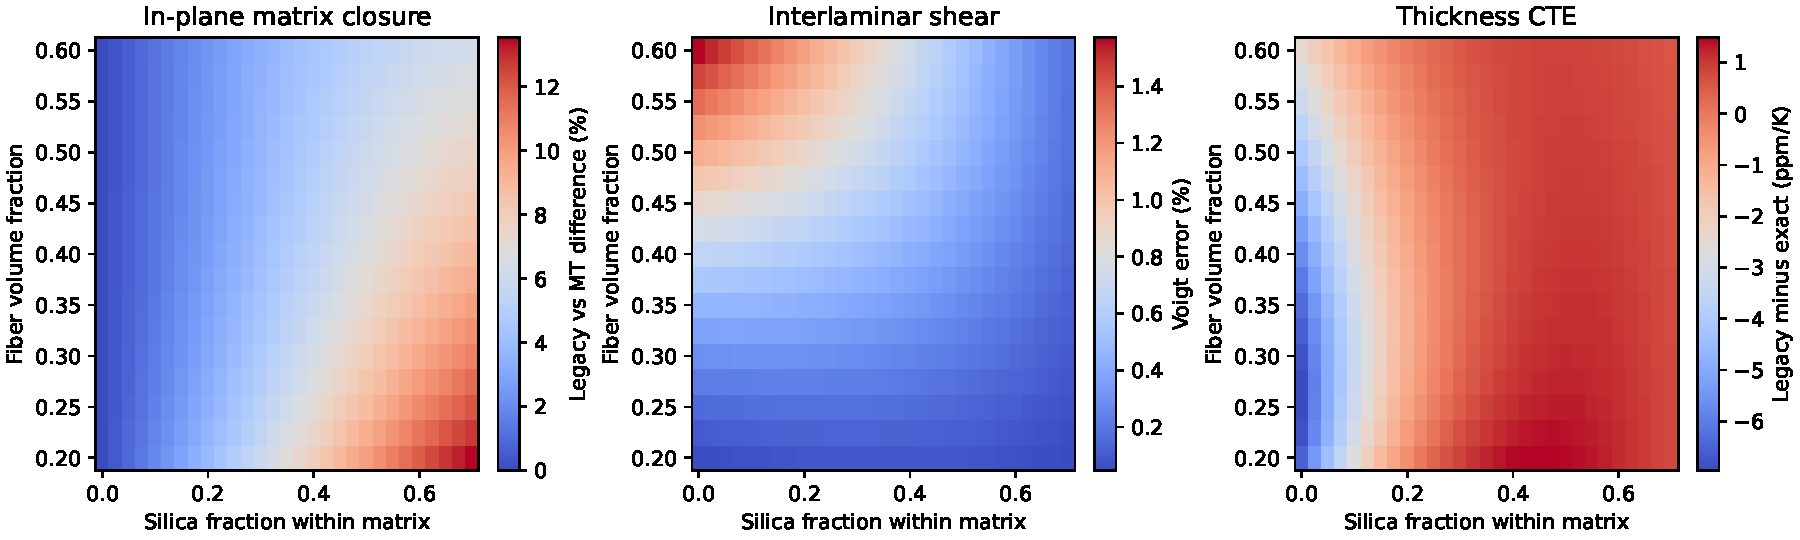
\includegraphics[width=\textwidth]{../results/figures/model_error_map.pdf}
\caption{Composition-dependent closure and script errors. Silica fraction
is within the non-fiber matrix.}
\end{figure}

\section{Discussion and limitations}
The dominant numerical sensitivity in this idealized family is the
filled-matrix stiffness closure. High-loading silica/epoxy studies report
model deviations and particle-shape effects \cite{ref5,ref29,ref28}; the
0.70 nested silica input needs a defined packing \cite{ref27}. Resin cure,
temperature dependence, interfaces, porosity, and woven reinforcement are
omitted. No matched measurement validates either closure or the final
laminate predictions. The code therefore supplies a verified audit rather
than a submission-ready original physical finding.

\bibliographystyle{unsrt}
\bibliography{references}
\end{document}
